\documentclass[slidestop,compress,mathserif]{beamer}
%\usepackage[bars]{beamerthemetree} % Beamer theme v 2.2
%\usetheme{Antibes}
\usetheme{Copenhagen}
%\usetheme{Dresden}
%\usetheme{JuanLesPins}
%\usetheme{Boadilla}
%\usetheme{Rochester} %sobrio
% Beamer theme v 3.0
%\usecolortheme{lily}
%\usecolortheme{albatross}
%\usecolortheme{seahorse}
%\usecolortheme{beetle}
%\usecolortheme{crane}
%\usecolortheme{dolphin}
%\usecolortheme{dove}
%\usecolortheme{fly}
%\usecolortheme{lily}
%\usecolortheme{orchid}
%\usecolortheme{rose}
%\usecolortheme{seagull}
\usecolortheme{whale}

%\usepackage{bbding}
\usepackage{pifont}
%\usepackage{fourier-orns}

\usepackage{tabularx}
\usepackage{color}

\newcommand{\cmark}{\ding{51}}
\newcommand{\xmark}{\ding{55}}

\setbeamertemplate{navigation symbols}{}
\setbeamertemplate{footline}
{
  \leavevmode
  \hbox{
    \begin{beamercolorbox}
      [wd=.5\paperwidth,ht=2.5ex,dp=1.125ex,leftskip=.3cm plus1fill,rightskip=.3cm]
      {author in head/foot}
      \usebeamerfont{author in head/foot}\insertauthor
    \end{beamercolorbox}%
    \begin{beamercolorbox}[wd=.5\paperwidth,ht=2.5ex,dp=1.125ex,leftskip=.3cm,rightskip=.3cm plus1fill]
      {title in head/foot}%
      \usebeamerfont{title in head/foot}\insertshortinstitute
  \end{beamercolorbox}}%
  \vskip0pt%
}

%\beamertemplateshadingbackground{blue!20}{white!40}
%\setbeamercolor{title}{fg=red!80!black,bg=red!20!white}
%\setbeamercolor{navigation symbols dimmed}{fg=red!80!black}
%\setbeamercolor{navigation symbols}{fg=red!80!black}

%COLORES DEL TITULO
%\setbeamercolor*{palette tertiary}{fg=white,bg=structure.black!60!green}
%\setbeamercolor*{palette secondary}{fg=white,bg=structure.black!50!green}
%\setbeamercolor*{palette primary}{use=structure,fg=white,bg=structure.black!40!green}
%\setbeamercolor{itemize item}{fg=red}

% Beamer color theme
\usepackage [utf8]{inputenc}

% General data
\title[Master Thesis and experiences]
{Free Software Master Thesis and experiences}
%\subtitle {Solamente si hay subtítulo}
\author[Autores abreviados]{Antonio Arias Losada}
\institute{Free Software Master - 2011/2012}


\begin{document}

\begin{frame}
  % Cover slide
  \titlepage
  \begin{center}
    
\includegraphics[height=1cm]{images/igalia.png}
    \hspace{10mm}
    
\includegraphics[height=1cm]{images/urjc.png}
  \end{center}
\end{frame}

\begin{frame}
  \frametitle{Table of contents}

  \tableofcontents[hideallsubsections]
\end{frame}


\section{Introduction}
\begin{frame}
  \frametitle{Introduction}

  Before...

  \begin{block}{}<2->
    Open source is something that I had been using since the University time, but without realizing everything that is behind it.
  \end{block}

  \begin{block}{}<3->
    Sometimes I had some doubts about licensing, but it didn't seem important to me.
  \end{block}

  \begin{block}{}<4->
    I used to think that contributing or starting a new open source project is just reserved for ``gurus''.
  \end{block}

  \begin{block}{}<5->
    I thought that open source had born with Linux.
  \end{block}
\end{frame}

\section{Master Thesis}
\begin{frame}
  \frametitle{Master Thesis}

  Title:
  \begin{center}
    \textit{Crosscompilation of the open source web browser engine WebKitGTK+ for the ARMv7 processors}
  \end{center}

  Author:
  Antonio Arias Losada

  Tutor:
  V\'ictor Manuel J\'aquez Leal

\end{frame}

\subsection{Objectives}
\begin{frame}
  \frametitle{Objectives}

  The main objective is \textbf{building} a Linux based \textbf{image} for \textbf{ARMv7} processors architecture with a \textbf{WebKit2} web browser fully functional.
  
  To achieve the main goal, the work was divided the following subobjectives:

  \vspace{5mm}

  \begin{enumerate}
    \item<2-> Compile WebKit.
    \item<3-> Prepare Yocto environment.
    \item<4-> Create a Yocto image for ARM and run it with QEMU.
    \item<5-> Create a Yocto image for ARM with WebKit.
  \end{enumerate}

\end{frame}

\subsection{Motivation}
\begin{frame}
  \frametitle{Motivation}

  This work is motivated basically by two key points:
  \pause

  \vspace{10mm}
  \begin{center}
    
\includegraphics[height=2.5cm]{images/HTML5-logo.png}
    \hspace{10mm}
    \pause
    \href{http://financialreports.arm.com/downloads/pdfs/ARM_AR11_Our_Story_v1.pdf}{
\includegraphics[height=1.3cm]{images/ARM-logo.png}}
    
    \pause
    \color{gray}{
      \begin{tabularx}{\textwidth}{Xl}
         & 95\% mobiles; 90\% HDD; 40\% TV \\
         & +121 licenses (849 in total) \\
         & 7.9 billion units shipped \\
         & Increasing tendencies \\
         & [ARM Annual Report 2011]
      \end{tabularx}
    }
  \end{center}

\end{frame}

\subsection{Results}
\begin{frame}
  \frametitle{Results}

  These are the results of the proposed tasks:

  \begin{block}{Task \#1}<2->
    \begin{tabularx}{\textwidth}{Xr}
      WebKit2 GTK+ compiled for AMD64 architecture. & \cmark \\
    \end{tabularx}
  \end{block}

  \begin{block}{Task \#2}<3->
    \begin{tabularx}{\textwidth}{Xr}
      Yocto environment prepared. & \cmark \\
    \end{tabularx}
  \end{block}

  \begin{block}{Task \#3}<4->
    \begin{tabularx}{\textwidth}{Xr}
      Generated and ran an ARM image. & \cmark \\
    \end{tabularx}
  \end{block}

  \begin{alertblock}{Task \#4}<5->
    \begin{tabularx}{\textwidth}{Xr}
      Compile WebKit2 GTK+ for ARM architecture. & \xmark \\
    \end{tabularx}
  \end{alertblock}
\end{frame}

\subsection{Conclusions}
\begin{frame}
  \frametitle{Conclusions}

  The Master Thesis work conclusions are:

  \begin{block}{}<2->
    Embedded systems and development tools learning.
  \end{block}

  \begin{block}{}<3->
    Inconvenience of fragmented work time.
  \end{block}

  \begin{block}{}<4->
    Long testing cycles.
  \end{block}

  \begin{block}{}<5->
    Initially wrong planned tests.
  \end{block}

  \begin{block}{}<6->
    Positive global evaluation of the practicum work.
  \end{block}
\end{frame}

\section{Experiences}
\subsection{Daily}
\begin{frame}
  \frametitle{Daily}
  
  %Daily use of open source software.
  
  %Diffusion of the open source culture, trying to support the respect for it and the respecto for the licenses.

  \vspace*{\fill}
  \begin{center}
    
\includegraphics[height=3cm]{images/Tux.png}
  \end{center}

\end{frame}

\subsection{MFS Open sessions 2011}
\begin{frame}
  \frametitle{MFS Open sessions 2011}
  Introductory talk about Open Source Hardware in the open sessions of the Free Software Master 2011 edition, collaborating with Xulio Coira.

  \begin{center}
    
\includegraphics[height=5cm]{images/ohw-logo.png}
  \end{center}

\end{frame}

\subsection{OSHWDEM 2012}
\begin{frame}
  \frametitle{OSHWDEM 2012}
  OSHWDEM 2012 celebrated in A Coru\~na, on 17/11/2012.

  \begin{center}
    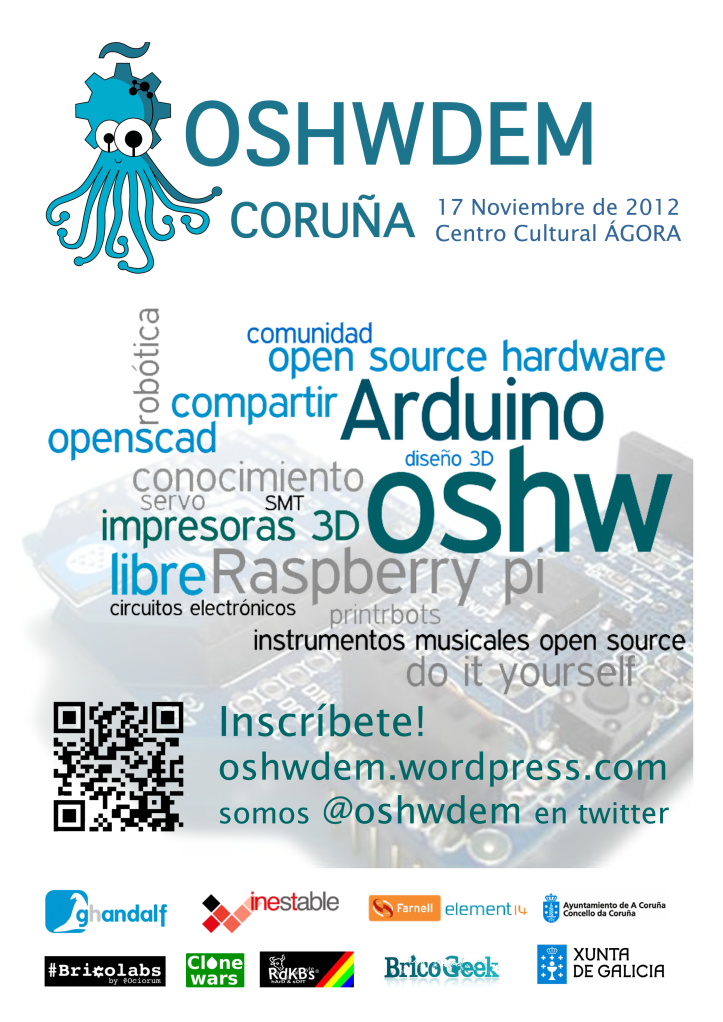
\includegraphics[height=6.5cm]{images/cartel-oshwdem5-300.png}
  \end{center}

\end{frame}

\subsection{Conclusion}
\begin{frame}
  \frametitle{Conclusion I}

  The main conclusions about my learning are:
  
  \begin{block}{FLOSS licenses}<2->
    Better understanding.\\
    A lot of myths dismantled.\\
    Learnt the importance of respecting them.
  \end{block}

  \begin{block}{FLOSS in the enterprise}<3->
    Knowledge about bussines models.\\
    Some myths dismantled.
  \end{block}

  \begin{block}{FLOSS communities}<4->
    How communities work.\\
    Technical dynamics of a project.
  \end{block}
\end{frame}

\begin{frame}
  \frametitle{Conclusion II}

  The main conclusions about my learning are:
  
  \begin{block}{Technologies}<1->
    Starting point to grow learning.
  \end{block}

  \begin{block}{Open source mind}<2->
    Changed the point of view about the open source.\\
    Started collaboration in open source project.\\
    Lost the fear to publish code.
  \end{block}

  \begin{block}{Networking}<3->
    Met a great group of classmates.
  \end{block}
\end{frame}

\section{}
\begin{frame}
  \vspace*{\fill}
  \begin{center}
    {\Huge Thank you!}
  \end{center}
\end{frame}

\begin{frame}
  \frametitle{License}
  This presentation is released under the following license:
  
  \begin{block}{}
    \begin{center}
      
\includegraphics[height=0.5cm]{images/cc-by.png}
  
      This work is licensed under a \href{http://creativecommons.org/licenses/by/3.0/deed.en_US}{Creative Commons Attribution 3.0 Unported License}.
    \end{center}
  \end{block}
\end{frame}

\begin{frame}
  \frametitle{Logo's licenses}
  \begin{tabularx}{\textwidth}{clX}
    \href{http://www.w3.org/html/logo/downloads/HTML5_Logo_512.png}{
\includegraphics[height=1cm]{images/HTML5-logo.png}} & HTML5 logo. & CC-By 3.0 \\
    \href{http://upload.wikimedia.org/wikipedia/commons/thumb/6/60/ARM_logo.svg/200px-ARM_logo.svg.png}{
\includegraphics[height=0.5cm]{images/ARM-logo.png}} & Similar ARM logo. & Public domain \\
    \href{http://upload.wikimedia.org/wikipedia/commons/a/af/Tux.png}{
\includegraphics[height=1cm]{images/Tux.png}} & Tux. & Explicit permission to use \\
    \href{http://oshwlogo.com/logos/ohw-logo.png}{
\includegraphics[height=1cm]{images/ohw-logo.png}} & OSHW logo. & Public domain \\    
  \end{tabularx}
\end{frame}

\end{document}
